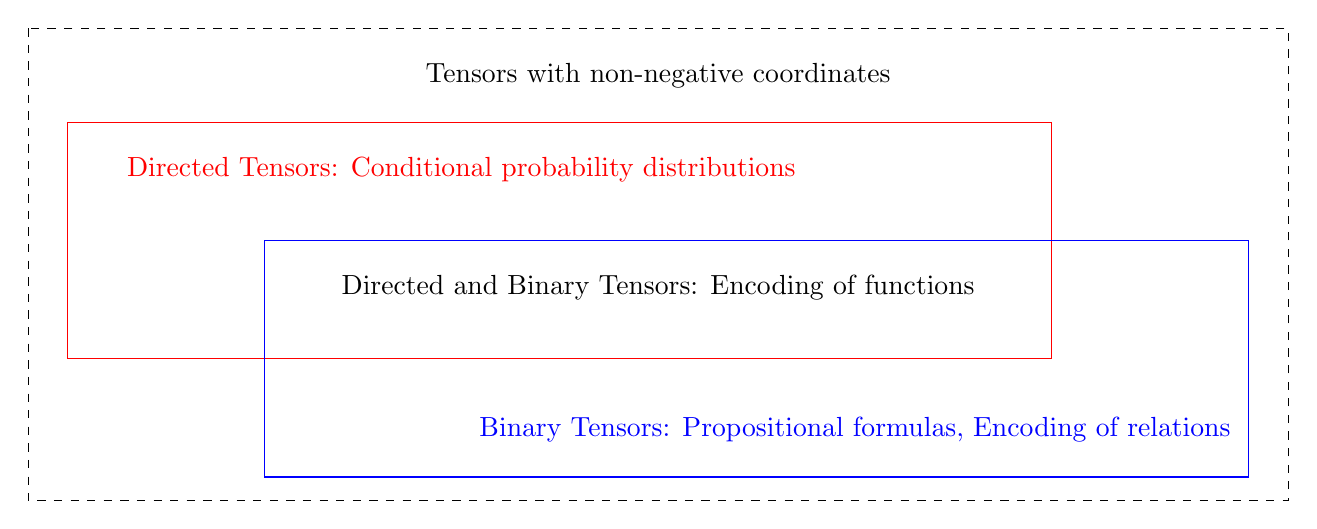
\begin{tikzpicture}[yscale=0.6]
	\draw[dashed] (-10.5,12) rectangle (5.5,2);
	\node[anchor=center] (text) at (-2.5,11) {Tensors with non-negative coordinates};
	
	\draw[red] (-10,10) rectangle (2.5,5); 
	\node[anchor=center,red] (text) at (-5,9) {Directed Tensors: Conditional probability distributions};
	\draw[blue] (-7.5,7.5) rectangle (5,2.5); 
	\node[anchor=center,blue] (text) at (0,3.5) {Binary Tensors: Propositional formulas, Encoding of relations};

	\node[anchor=center] (text) at (-2.5,6.5) {Directed and Binary Tensors: Encoding of functions};
\end{tikzpicture}